\documentclass[twocolumn,a4j]{jsarticle}
\setlength{\topmargin}{-20.4cm}
\setlength{\oddsidemargin}{-10.4mm}
\setlength{\evensidemargin}{-10.4mm}
\setlength{\textwidth}{18cm}
\setlength{\textheight}{26cm}

\usepackage[top=15truemm,bottom=25truemm,left=15truemm,right=15truemm]{geometry}
\usepackage[latin1]{inputenc}
\usepackage{amsmath}
\usepackage{amsfonts}
\usepackage{amssymb}
\usepackage[dvipdfmx]{graphicx}
\usepackage[dvipdfmx]{color}
\usepackage{listings}
\usepackage{listings,jvlisting}
\usepackage{geometry}
\usepackage{framed}
\usepackage{color}
\usepackage[dvipdfmx]{hyperref}
\usepackage{ascmac}
\usepackage{enumerate}
\usepackage{tabularx}
\usepackage{cancel}
\usepackage{scalefnt}

\renewcommand{\figurename}{Fig.}
\renewcommand{\tablename}{Table }

\lstset{
basicstyle={\ttfamily},
identifierstyle={\small},
commentstyle={\smallitshape},
keywordstyle={\small\bfseries},
ndkeywordstyle={\small},
stringstyle={\small\ttfamily},
frame={tb},
breaklines=true,
columns=[l]{fullflexible},
xrightmargin=0zw,
xleftmargin=3zw,
numberstyle={\scriptsize},
stepnumber=1,
numbersep=1zw,
lineskip=-0.5ex
}

\makeatletter
\def\@maketitle
{
\begin{center}
{\LARGE \@title \par}
\end{center}
\begin{flushright}
{\large 報告書 NO.08 - 1\quad\@date\quad\@author}
\end{flushright}
\par\vskip 1.5em
}
\makeatother

\setcounter{tocdepth}{3}

\author{来代 勝胤}
\title{令和3年度 12月 第1週 報告書}
\date{2021/12/2}

\begin{document}
\columnseprule=0.1mm

\maketitle
\section*{報告内容}
\begin{enumerate}[1.]
    \item 進捗状況
    \item 実験装置の製作
    \item 実験結果
    \item 実験装置のたわみ量とひずみの算出
    \item ひずみゲージの選定について
\end{enumerate}

\section{進捗状況}
実験装置のたわみ量とひずみセンサ取付部のひずみ量について
材料力学の理論から算出した.

\section{実験装置の製作}
作用力方向の違いによる影響を調べるため,
現在の実験装置を用いて仮実験を行うこととした.
仮実験を行うにあたり,以下のFig.19 の実験装置を作成した.
\begin{figure}[htbp]
    \footnotesize
    \begin{center}
        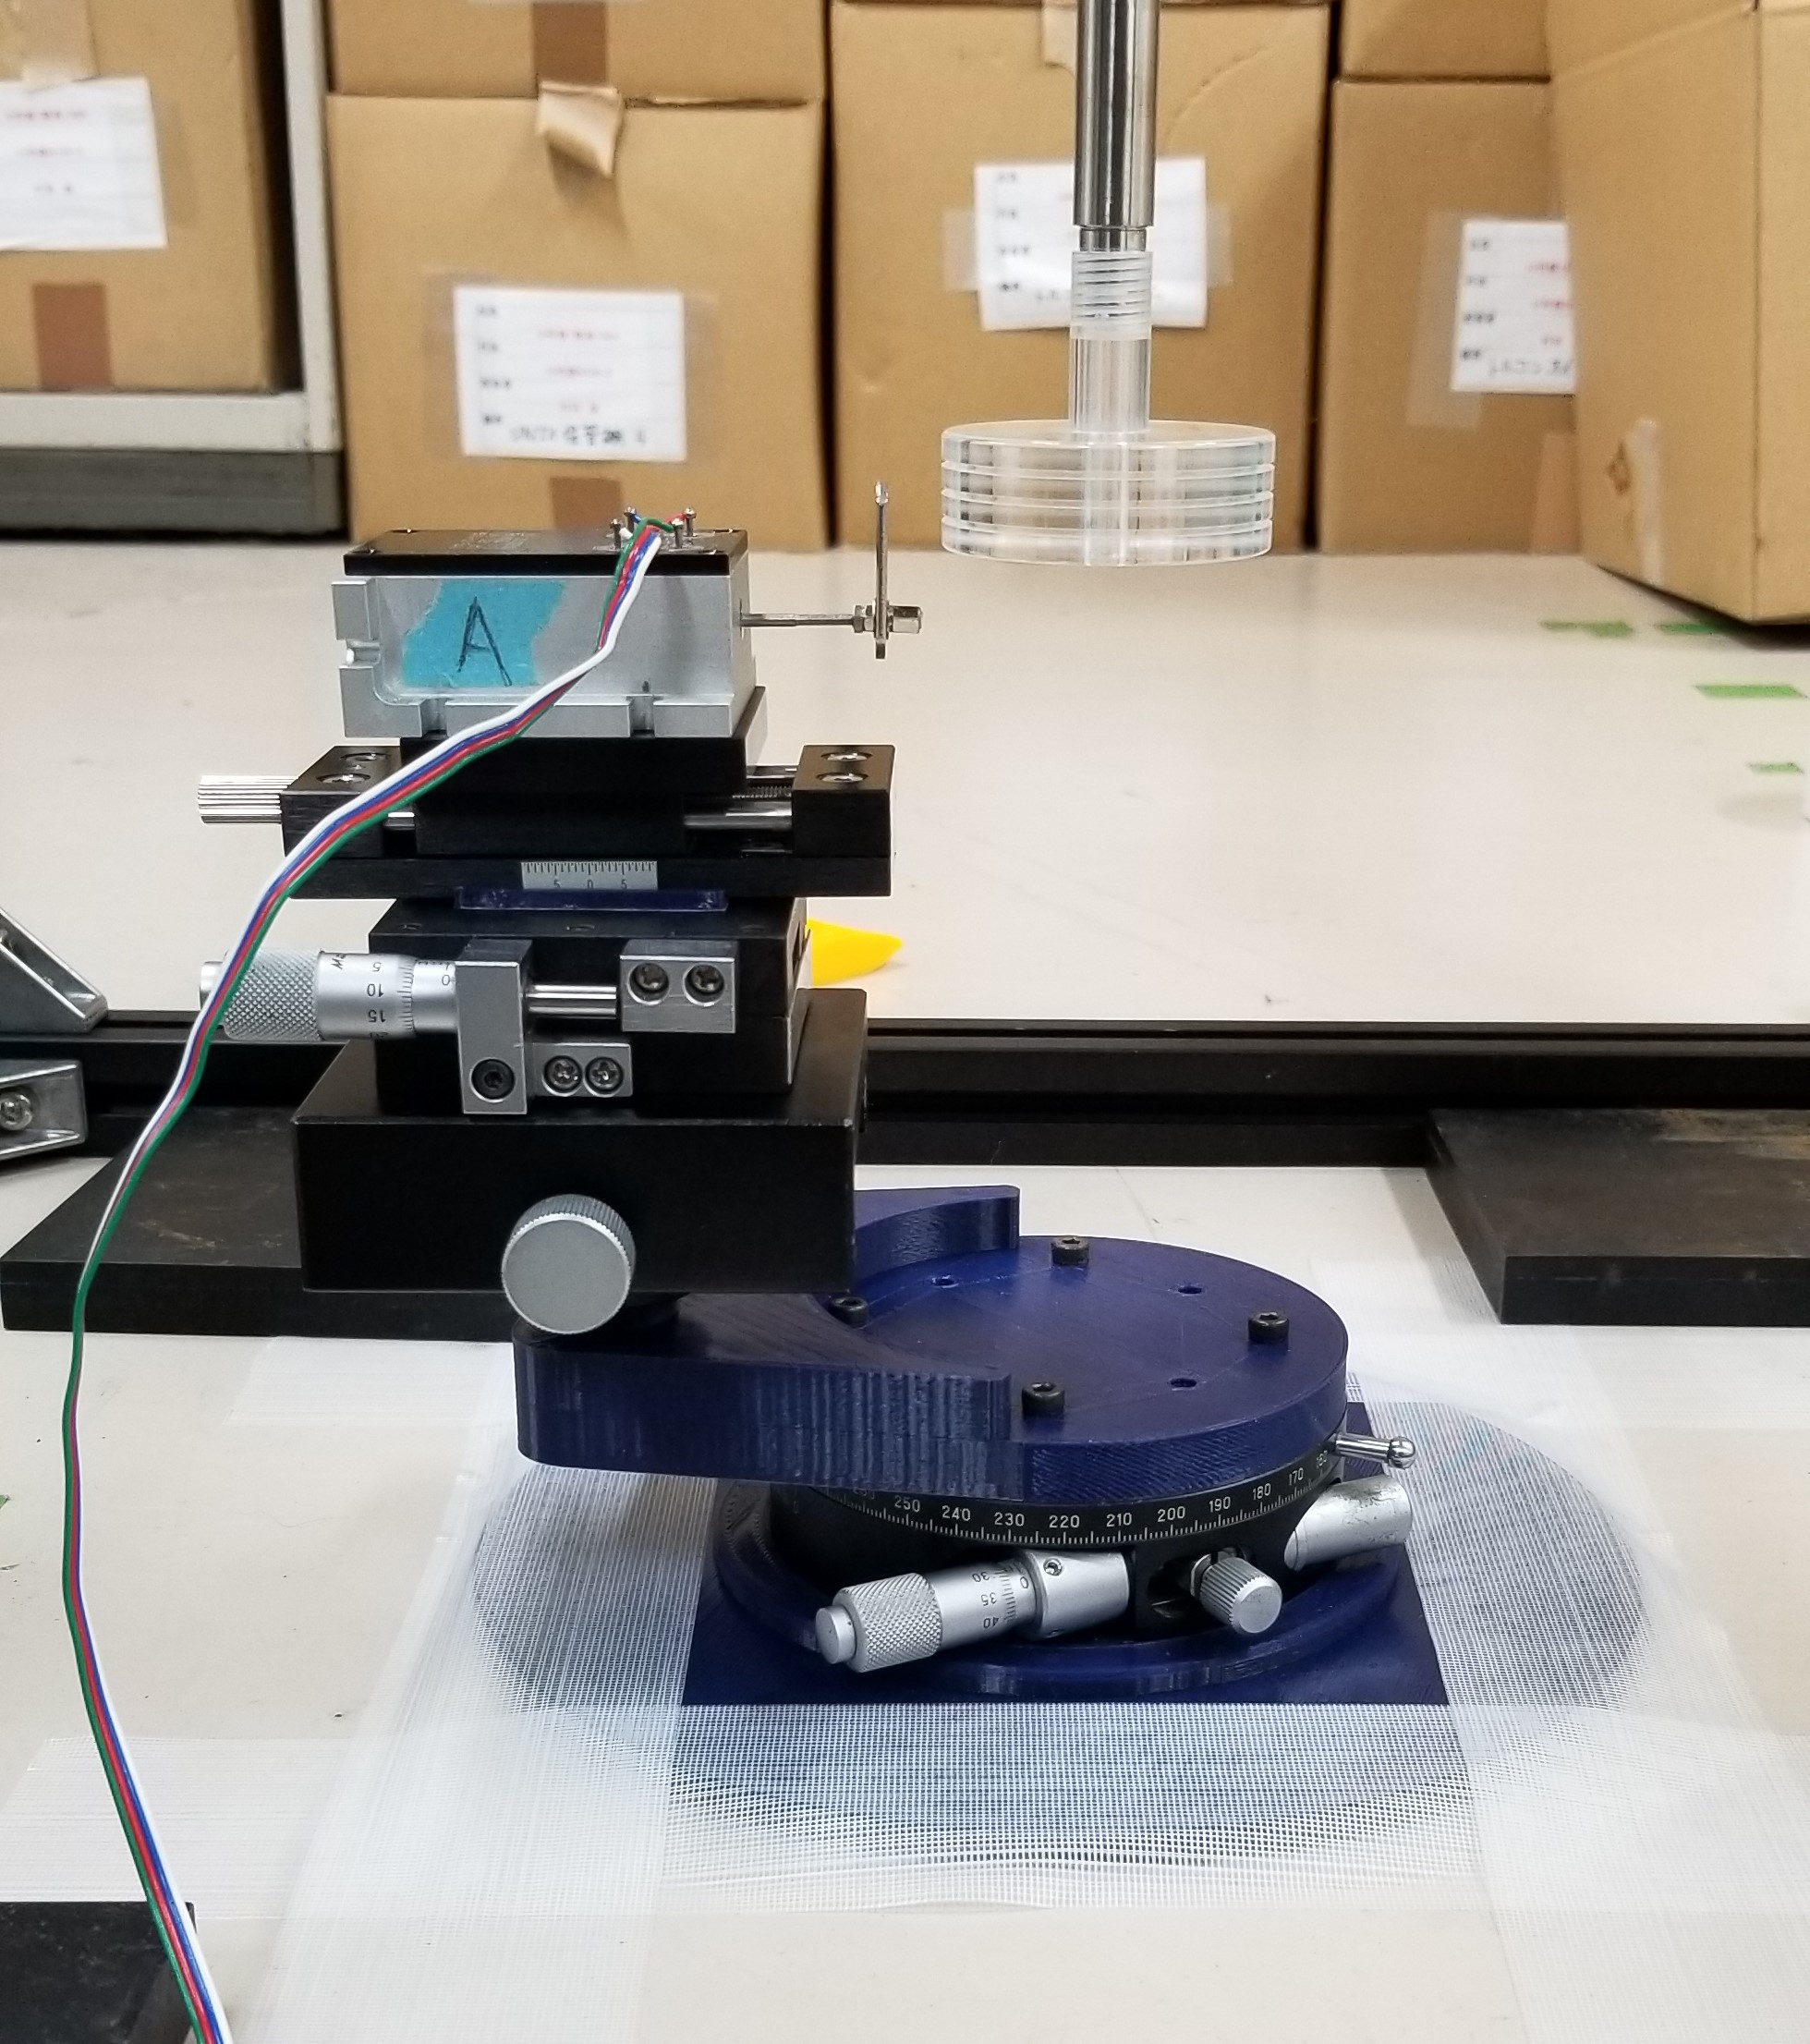
\includegraphics[width=65mm]{../images/device_1.jpg}
        \caption{Experimental device}
    \end{center}
\end{figure}

実験装置の概要は,以下のFig.20,Fig.21のとおりである.
角度を設定することのできる回転台とロードセルを
3Dプリンタで製作したジョイントを用いて固定している.

\begin{figure}[htbp]
    \footnotesize
    \begin{center}
        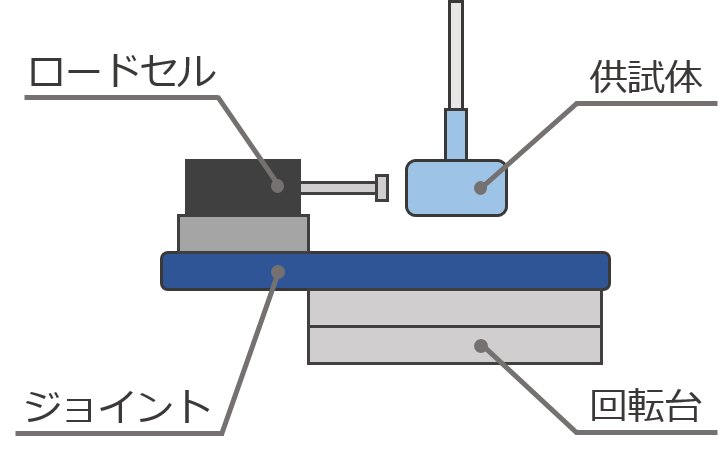
\includegraphics[width=65mm]{../images/rotation.png}
        \caption{Schematic of experimental device (side view)}
        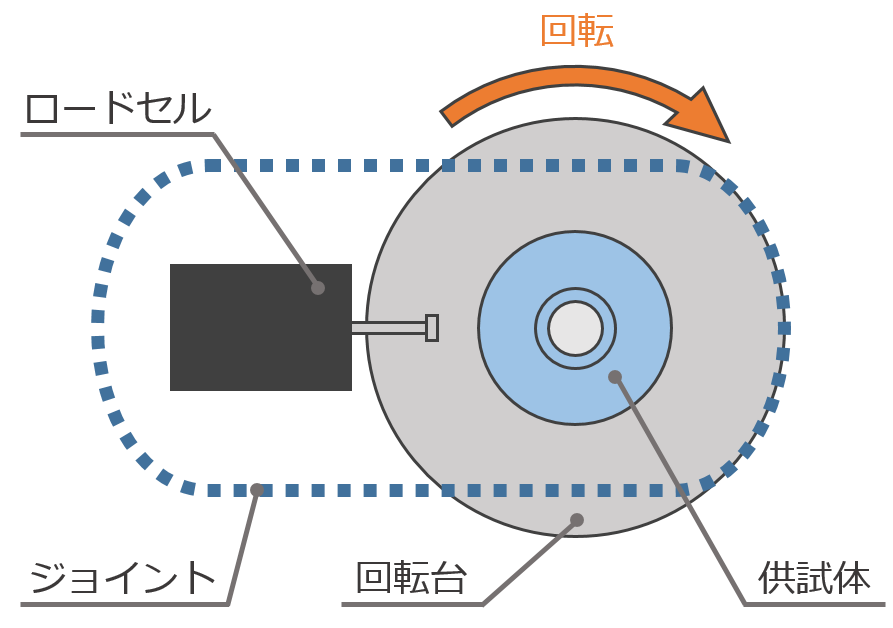
\includegraphics[width=70mm]{../images/rotation_2.png}
        \caption{Schematic of experimental device (top view)}
    \end{center}
\end{figure}

\newpage

\section{実験結果}
製作した実験装置を用いて,試験的に実験を行った.
その結果を以下に示す.
今回は,30度ずつ作用力方向を変化させ
計12回の測定を行った.
グラフにプロットしている値は,校正実験の再実施結果と同様に
採用点とその後9秒間の計10秒間の平均値を使用している.
また,ロードセルの出力電圧に関して,
オフセット値を測定開始前30秒間の平均値とし,
測定結果に適用している.

\begin{figure}[htbp]
    \footnotesize
    \begin{center}
        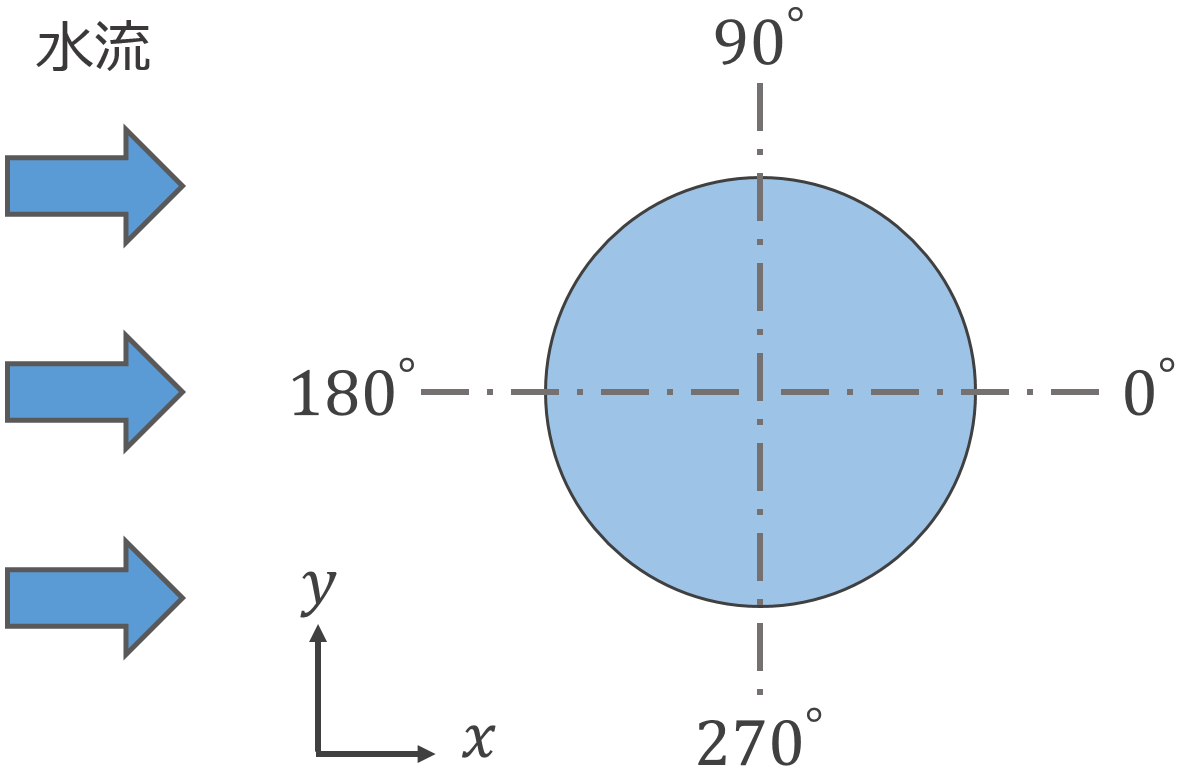
\includegraphics[width=58mm]{../images/model_1.png}
        \caption{Axis of experimental equipment}
    \end{center}
\end{figure}

\subsection{各角度における測定結果}
以下のFig.23 ~ Fig.34に各角度におけるひずみセンサの出力電圧の測定結果を示す.

\begin{figure}[htbp]
    \footnotesize
    \begin{center}
        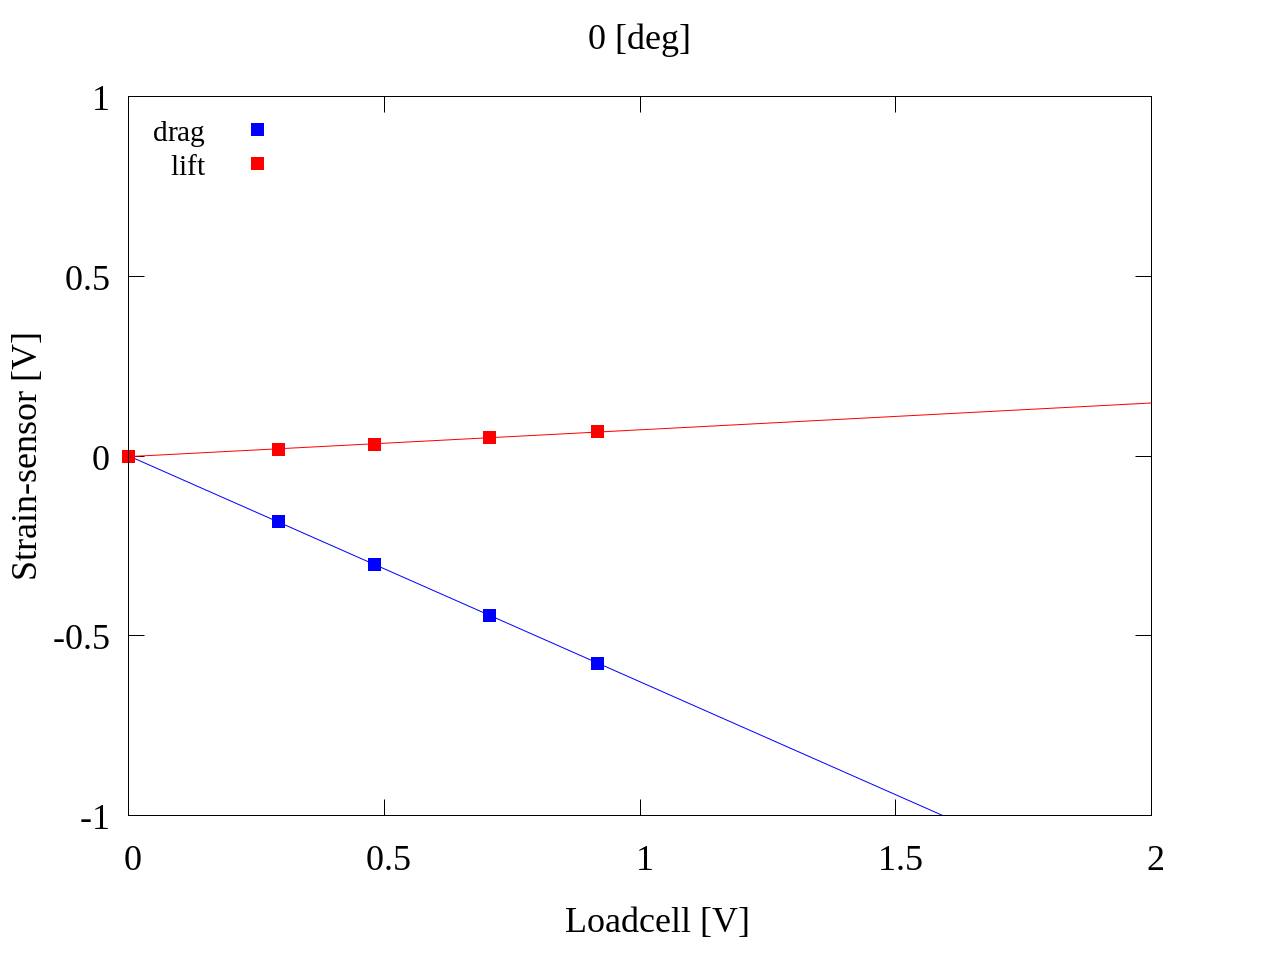
\includegraphics[width=78mm]{../images/0.png}
        \caption{Acting force from 0 degree direction}
        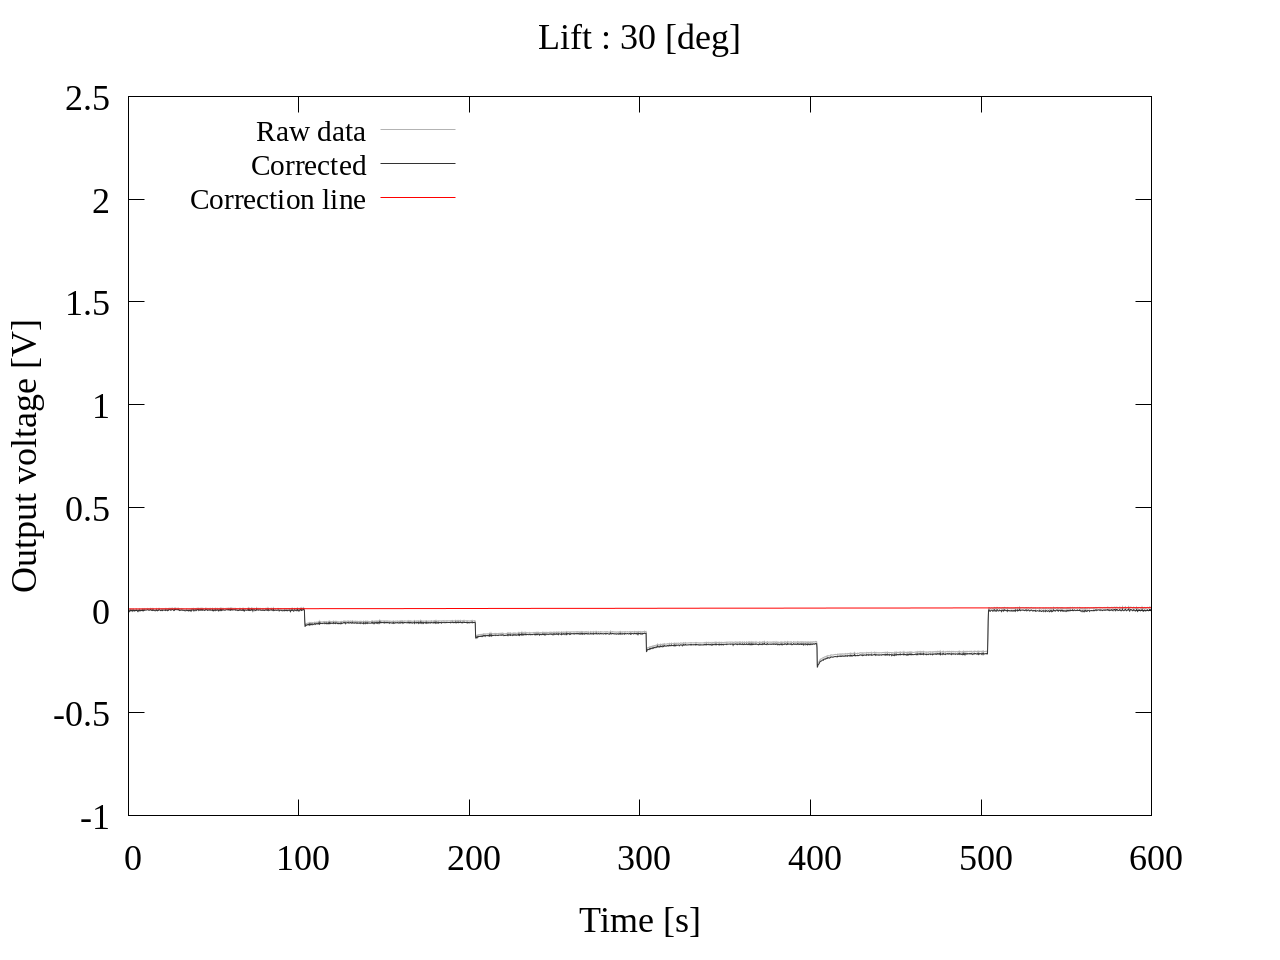
\includegraphics[width=78mm]{../images/30.png}
        \caption{Acting force from 30 degree direction}
    \end{center}
\end{figure}

\begin{figure}[htbp]
    \footnotesize
    \begin{center}
        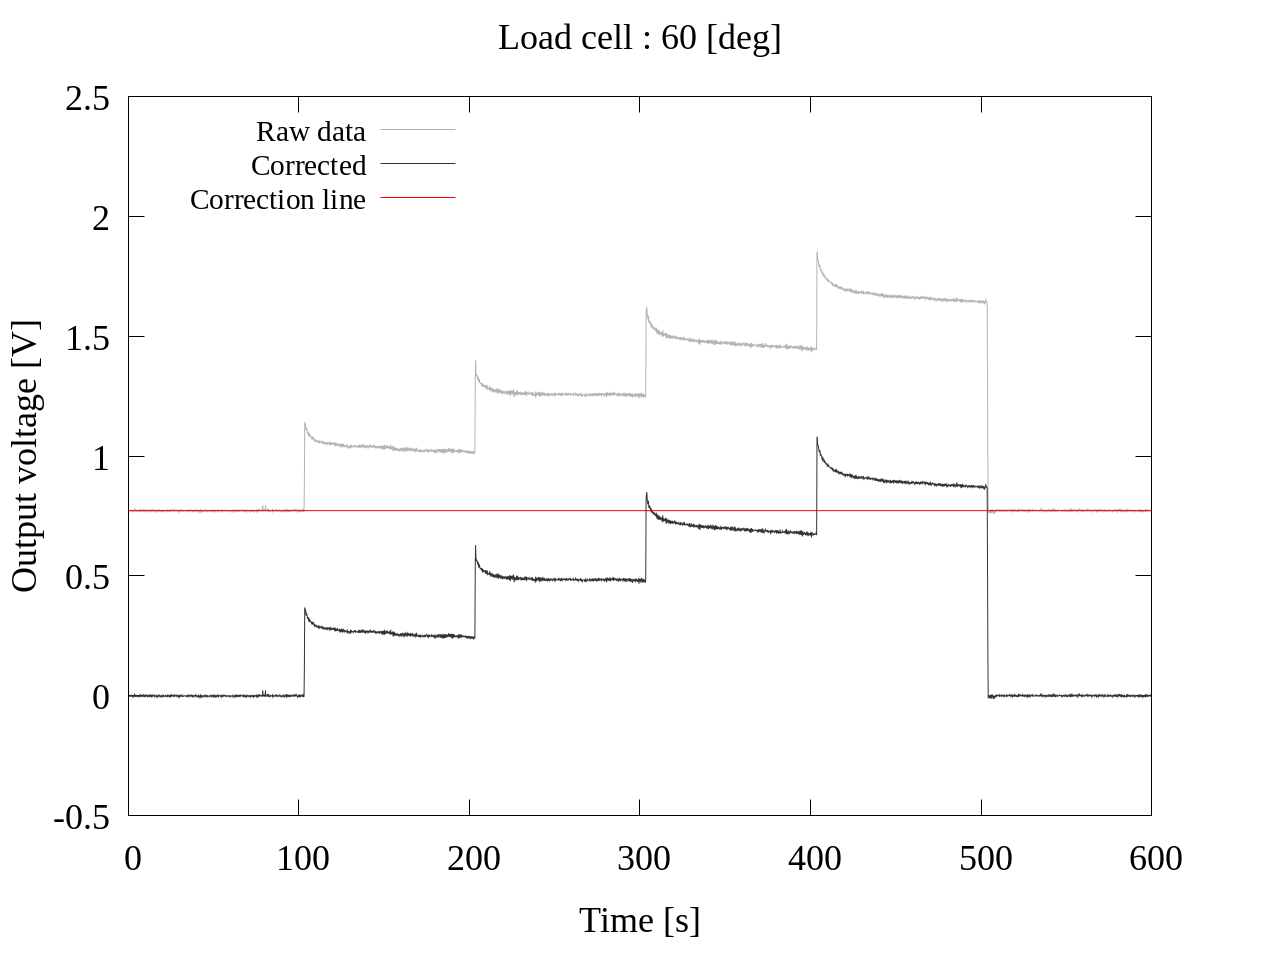
\includegraphics[width=78mm]{../images/60.png}
        \caption{Acting force from 60 degree direction}
        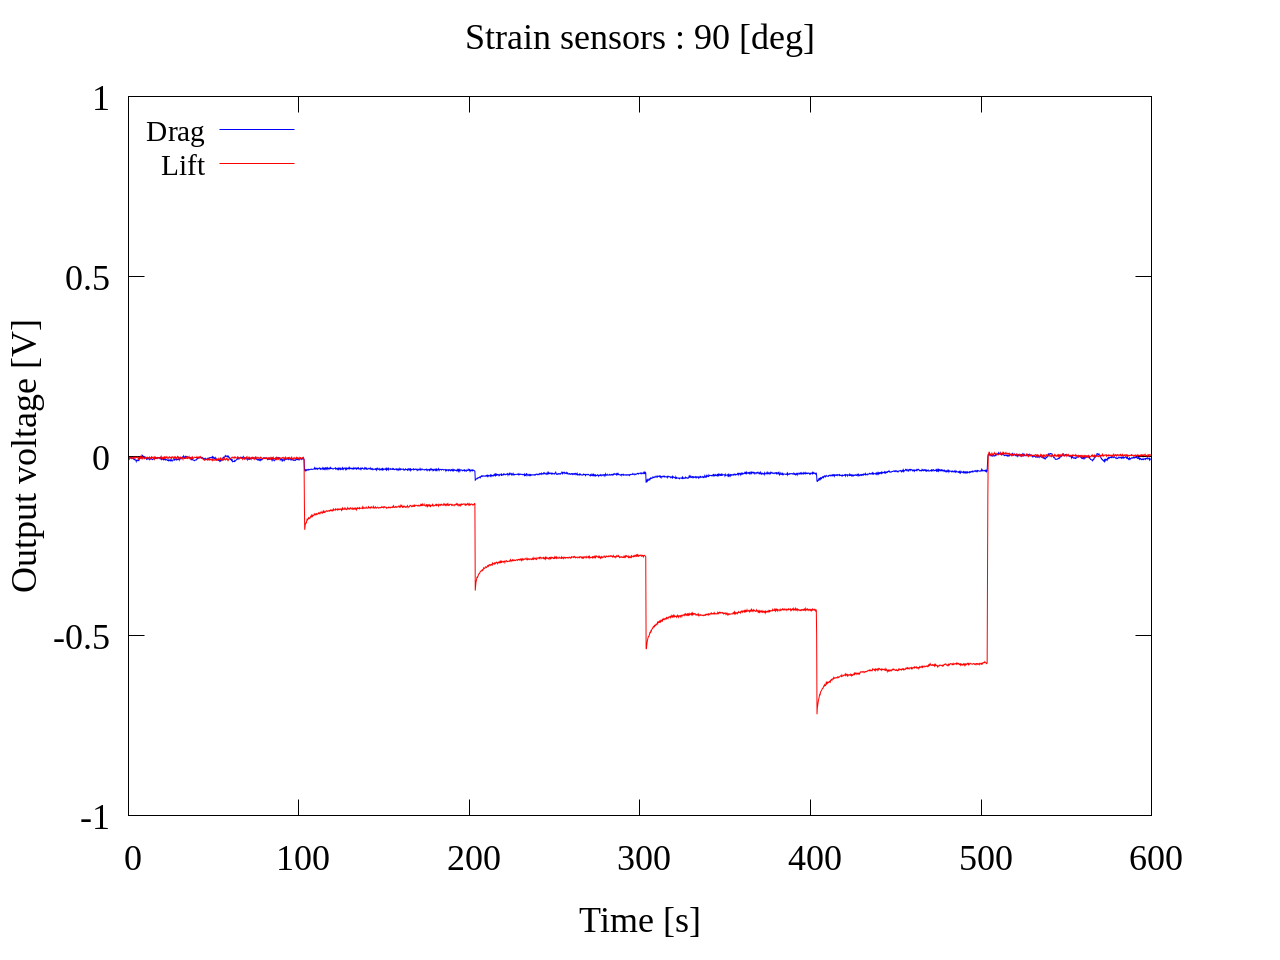
\includegraphics[width=78mm]{../images/90.png}
        \caption{Acting force from 90 degree direction}
        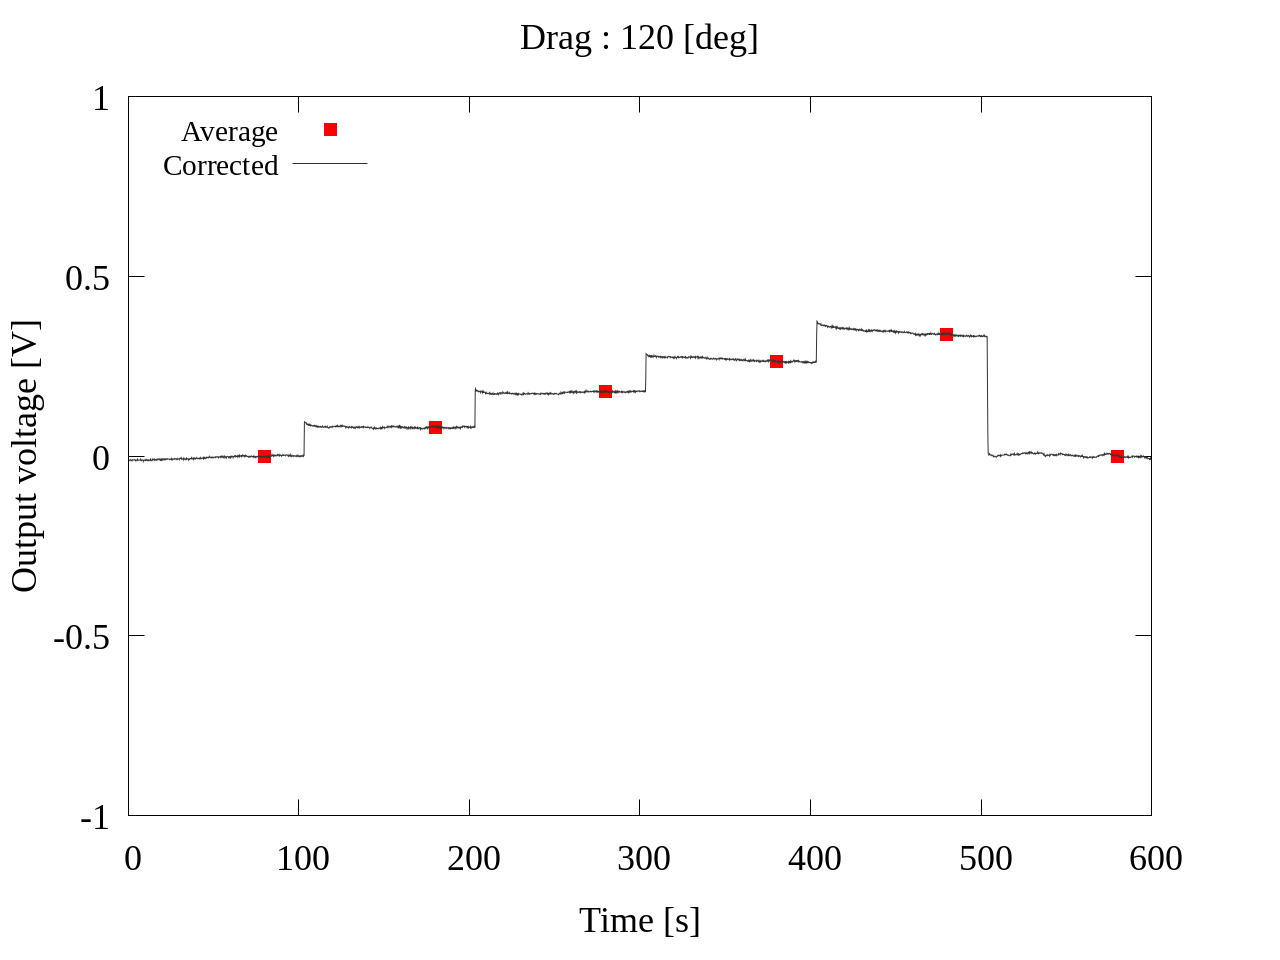
\includegraphics[width=78mm]{../images/120.png}
        \caption{Acting force from 120 degree direction}
        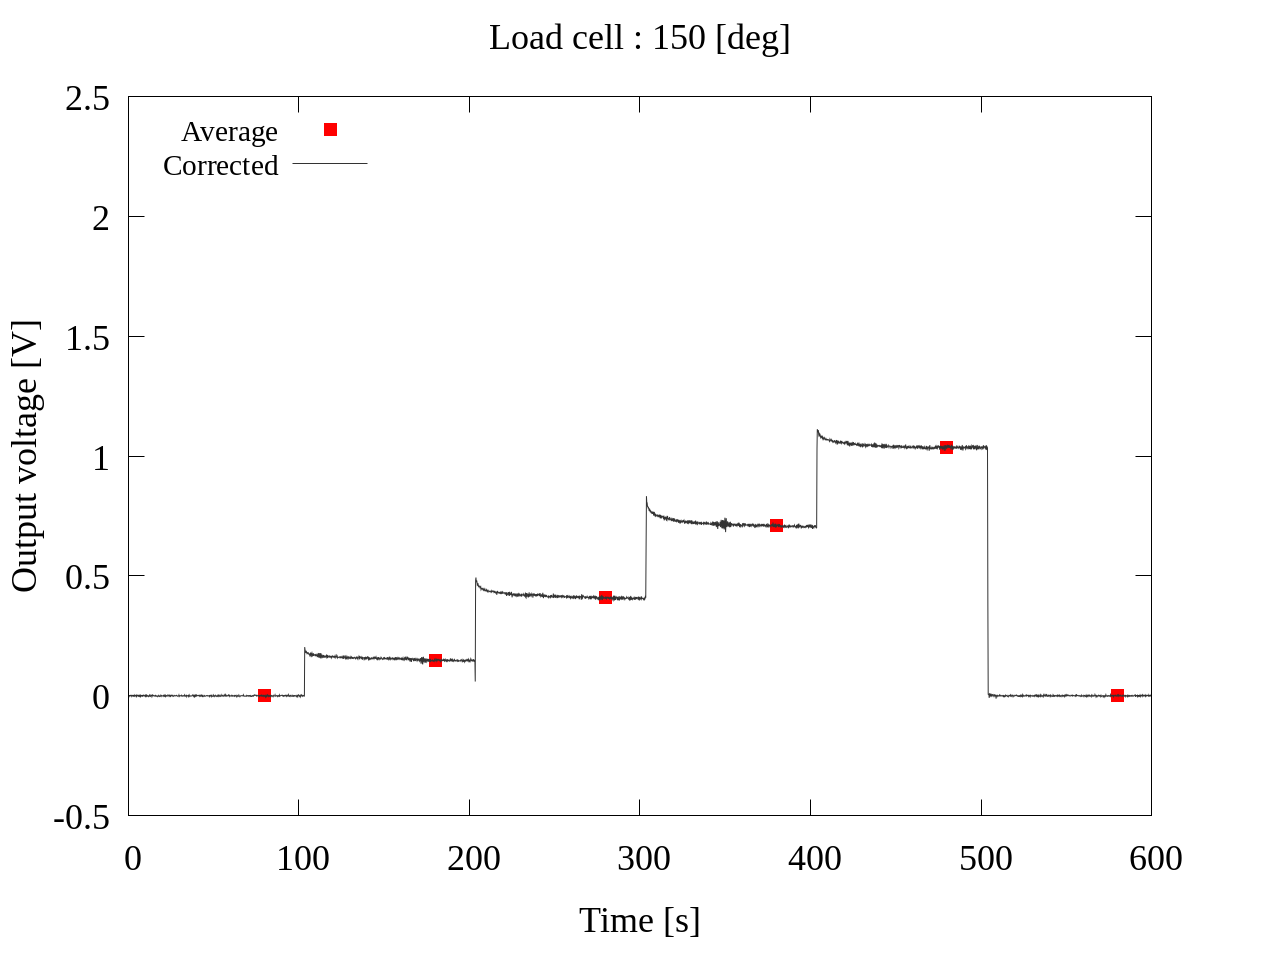
\includegraphics[width=78mm]{../images/150.png}
        \caption{Acting force from 150 degree direction}
    \end{center}
\end{figure}

\begin{figure}[htbp]
    \footnotesize
    \begin{center}
        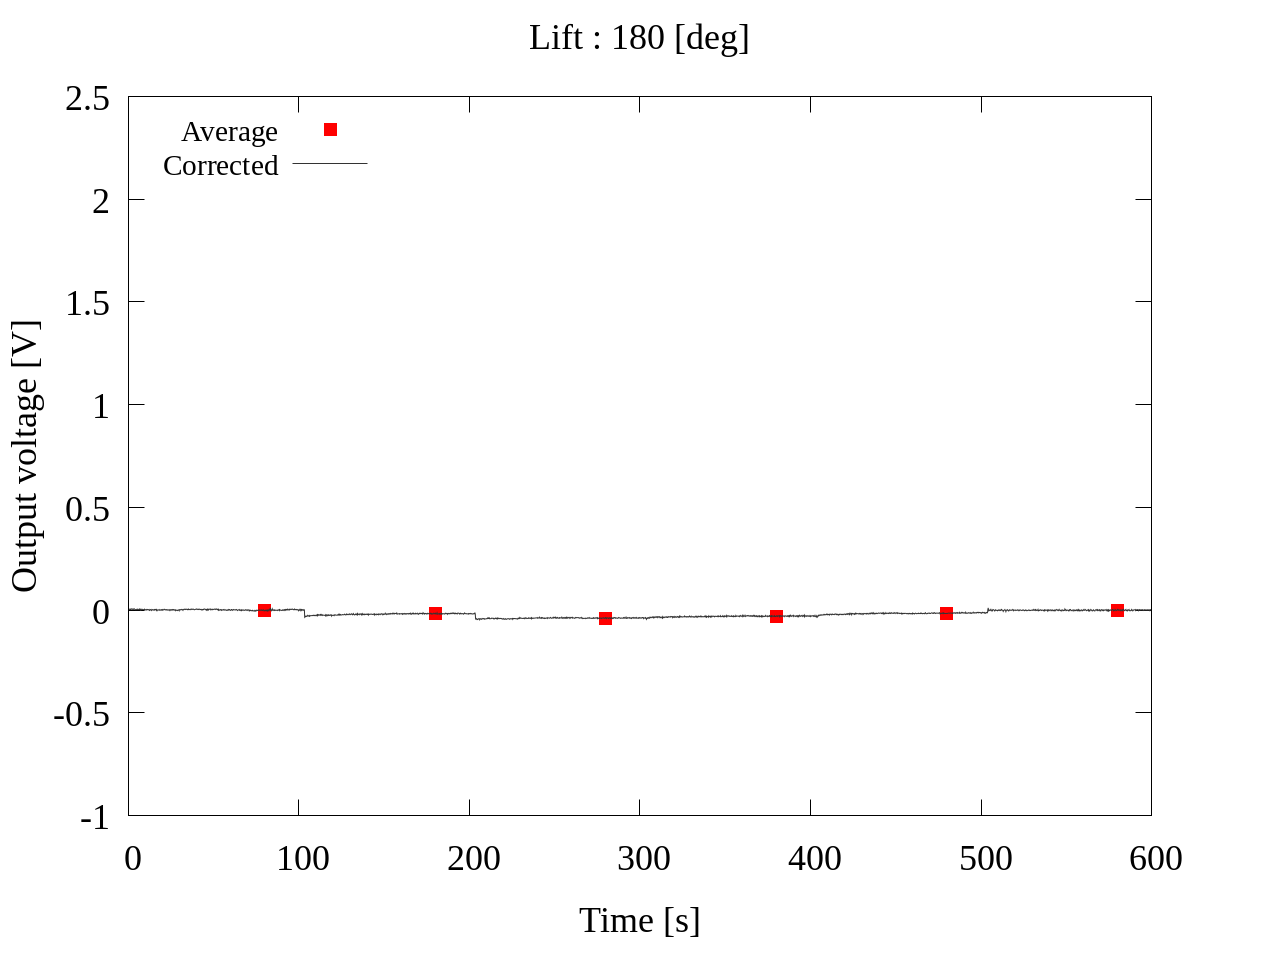
\includegraphics[width=78mm]{../images/180.png}
        \caption{Acting force from 180 degree direction}
        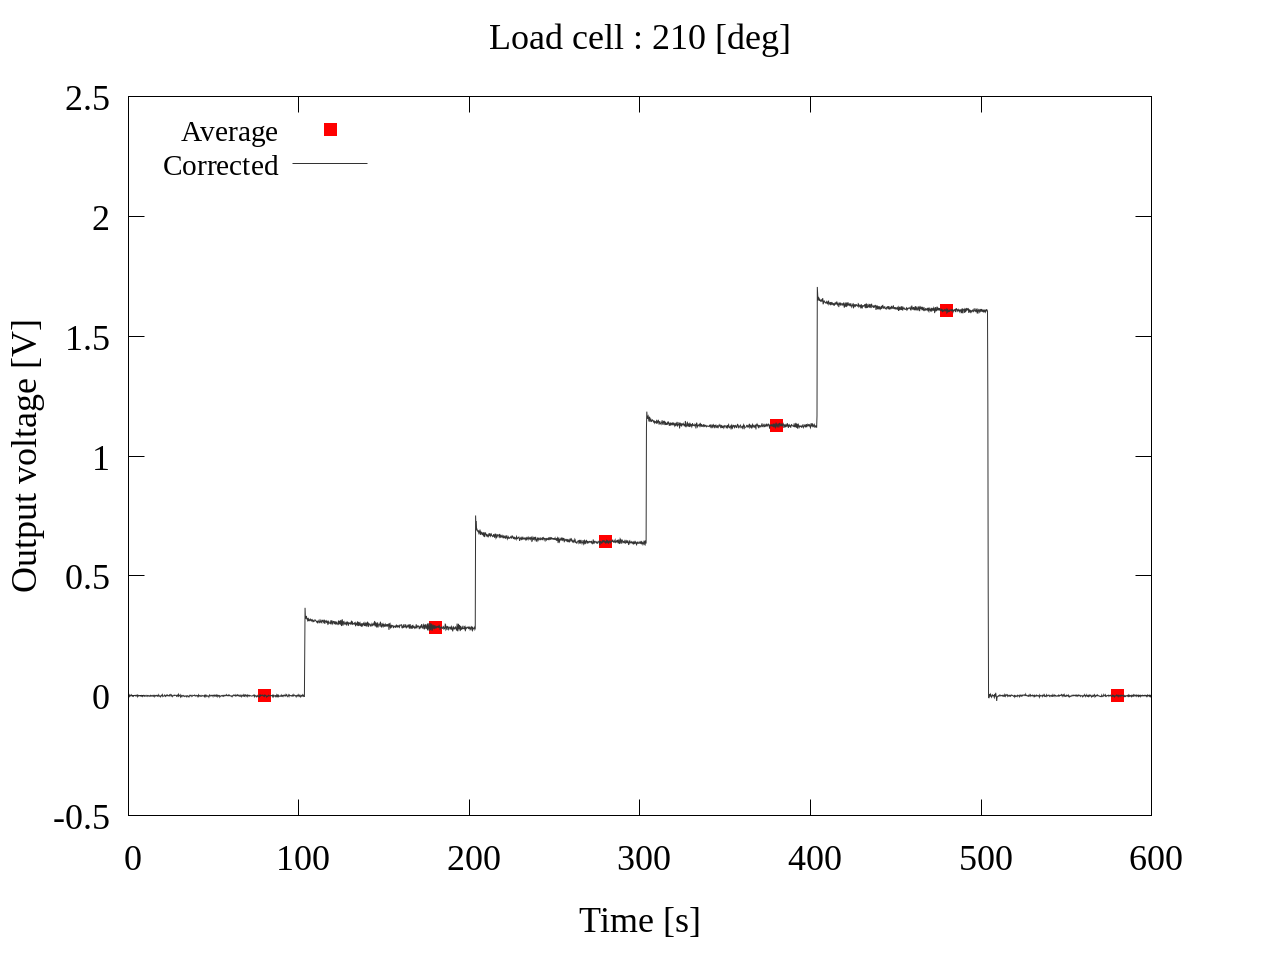
\includegraphics[width=78mm]{../images/210.png}
        \caption{Acting force from 210 degree direction}
        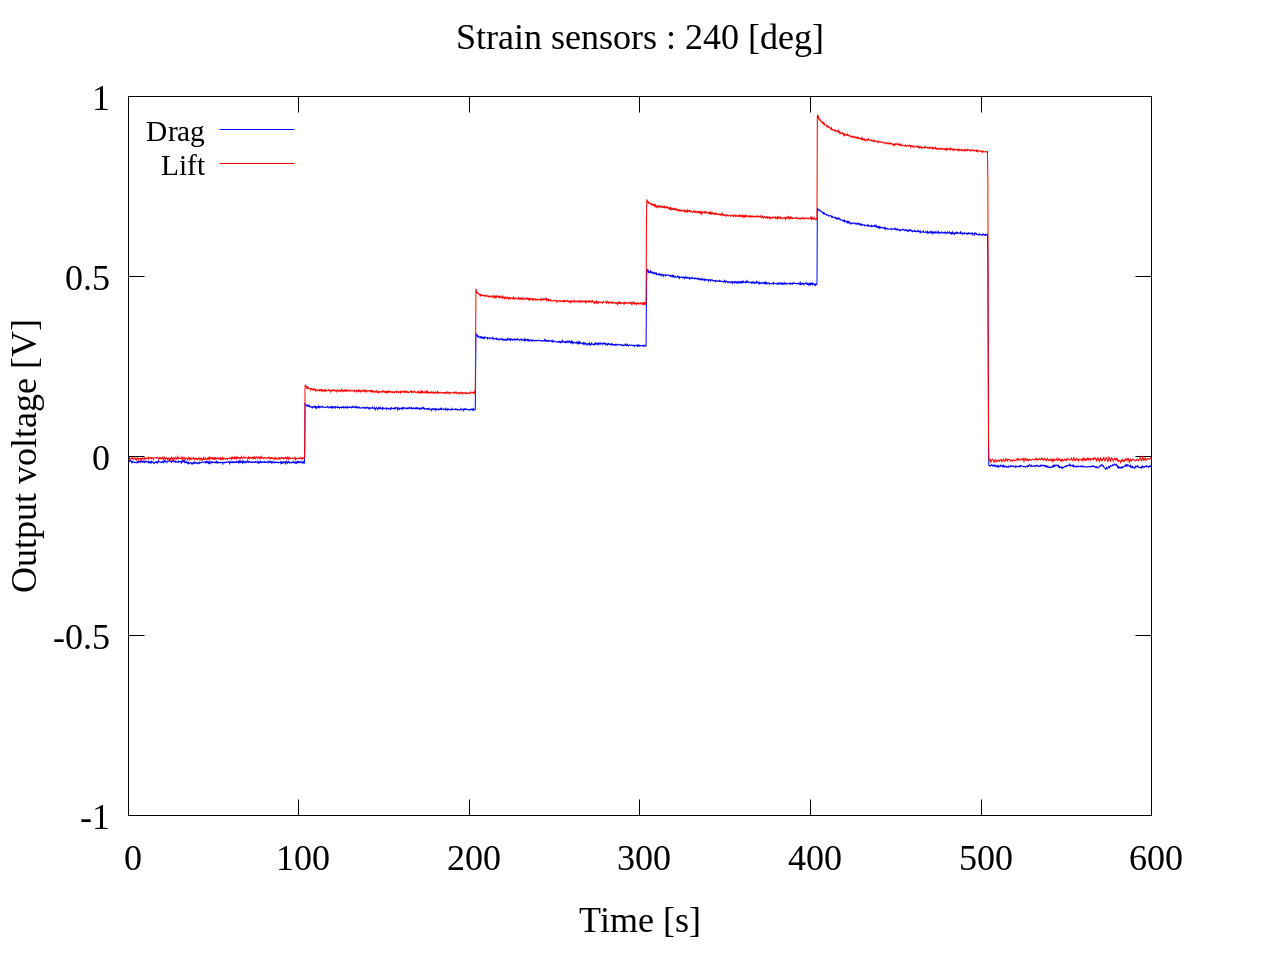
\includegraphics[width=78mm]{../images/240.png}
        \caption{Acting force from 240 degree direction}
    \end{center}
\end{figure}

\begin{figure}[htbp]
    \footnotesize
    \begin{center}
        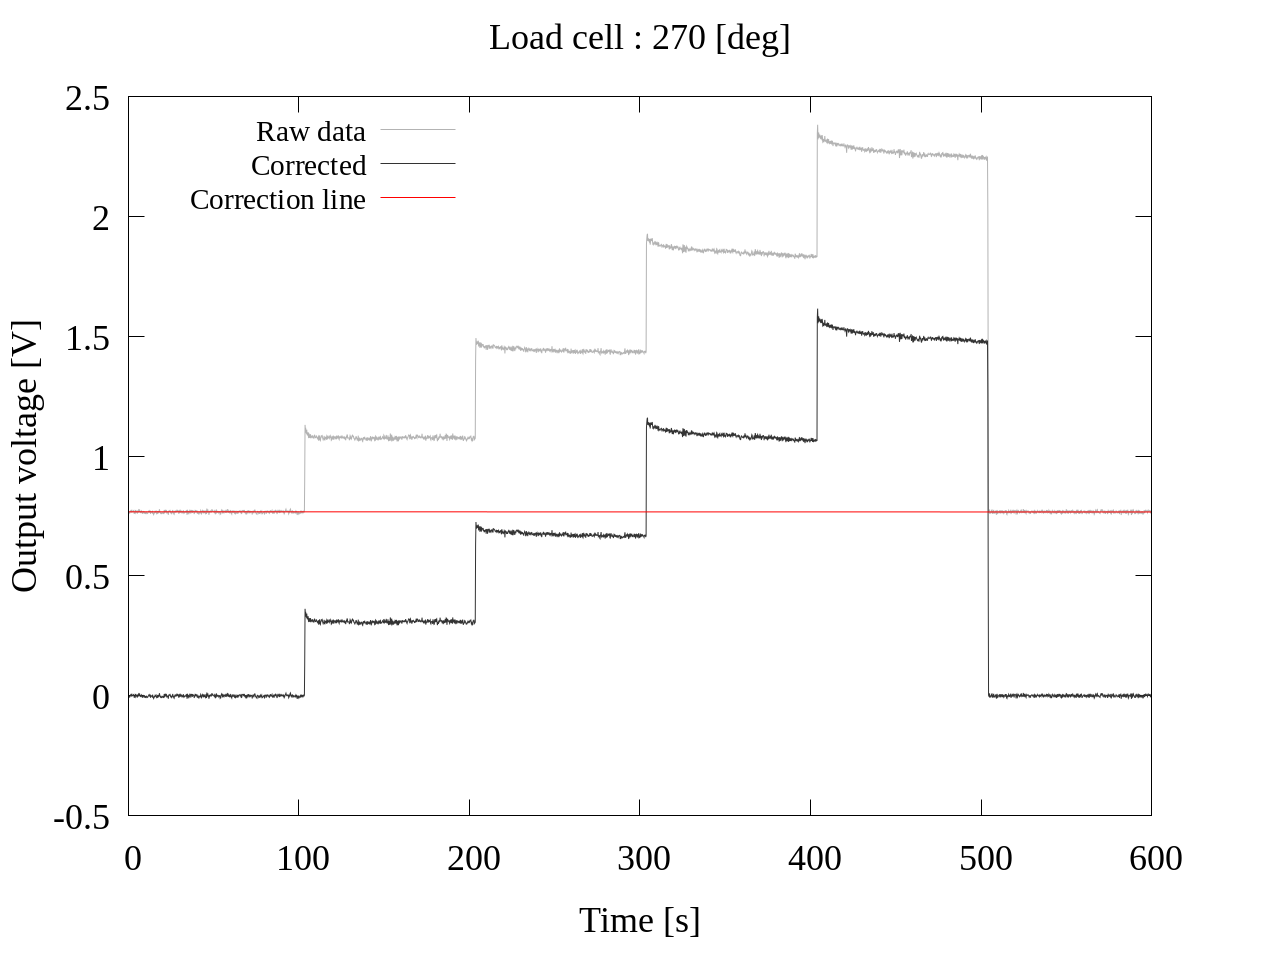
\includegraphics[width=78mm]{../images/270.png}
        \caption{Acting force from 270 degree direction}
        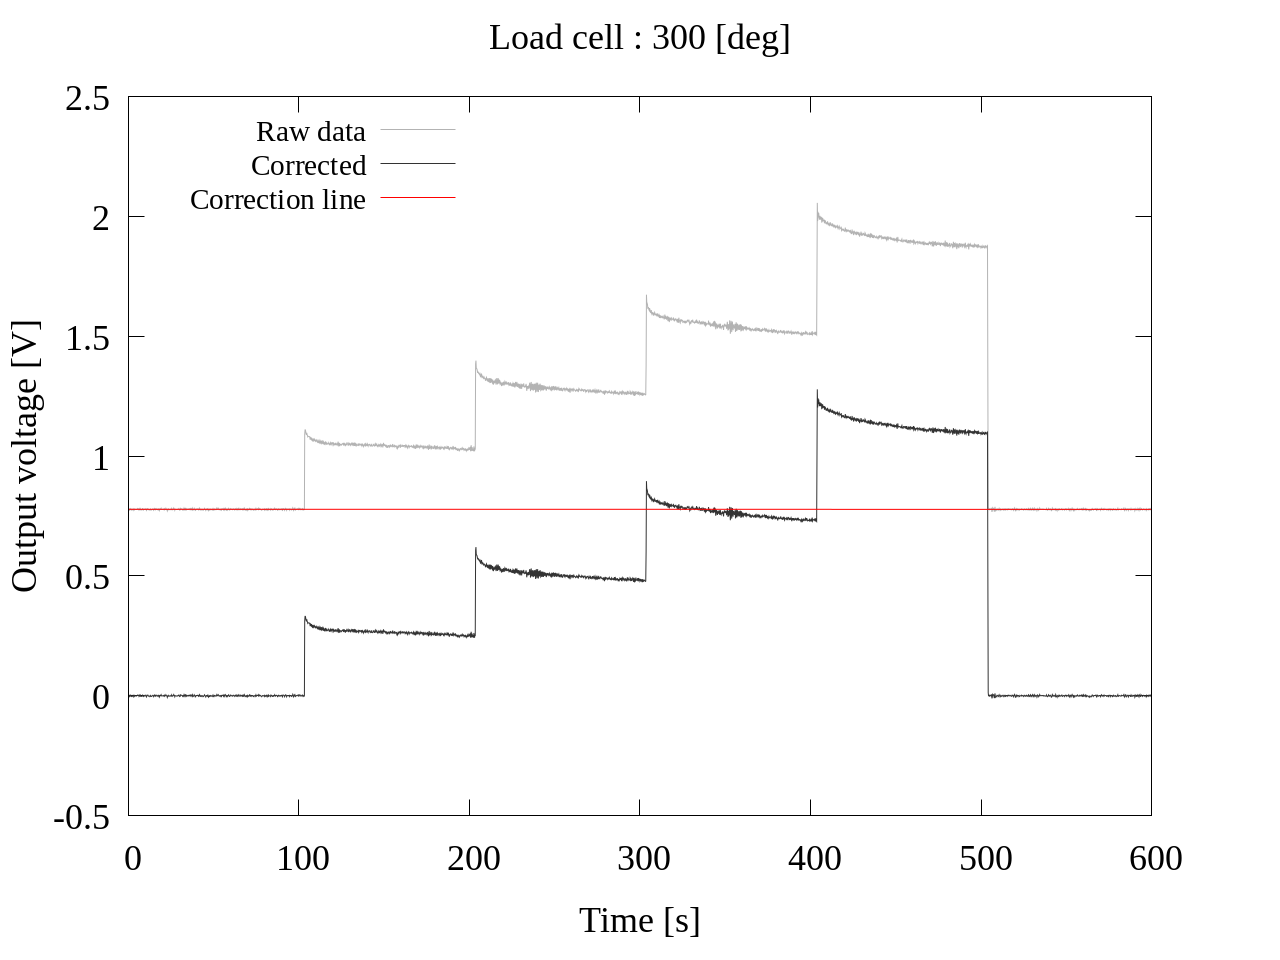
\includegraphics[width=78mm]{../images/300.png}
        \caption{Acting force from 300 degree direction}
        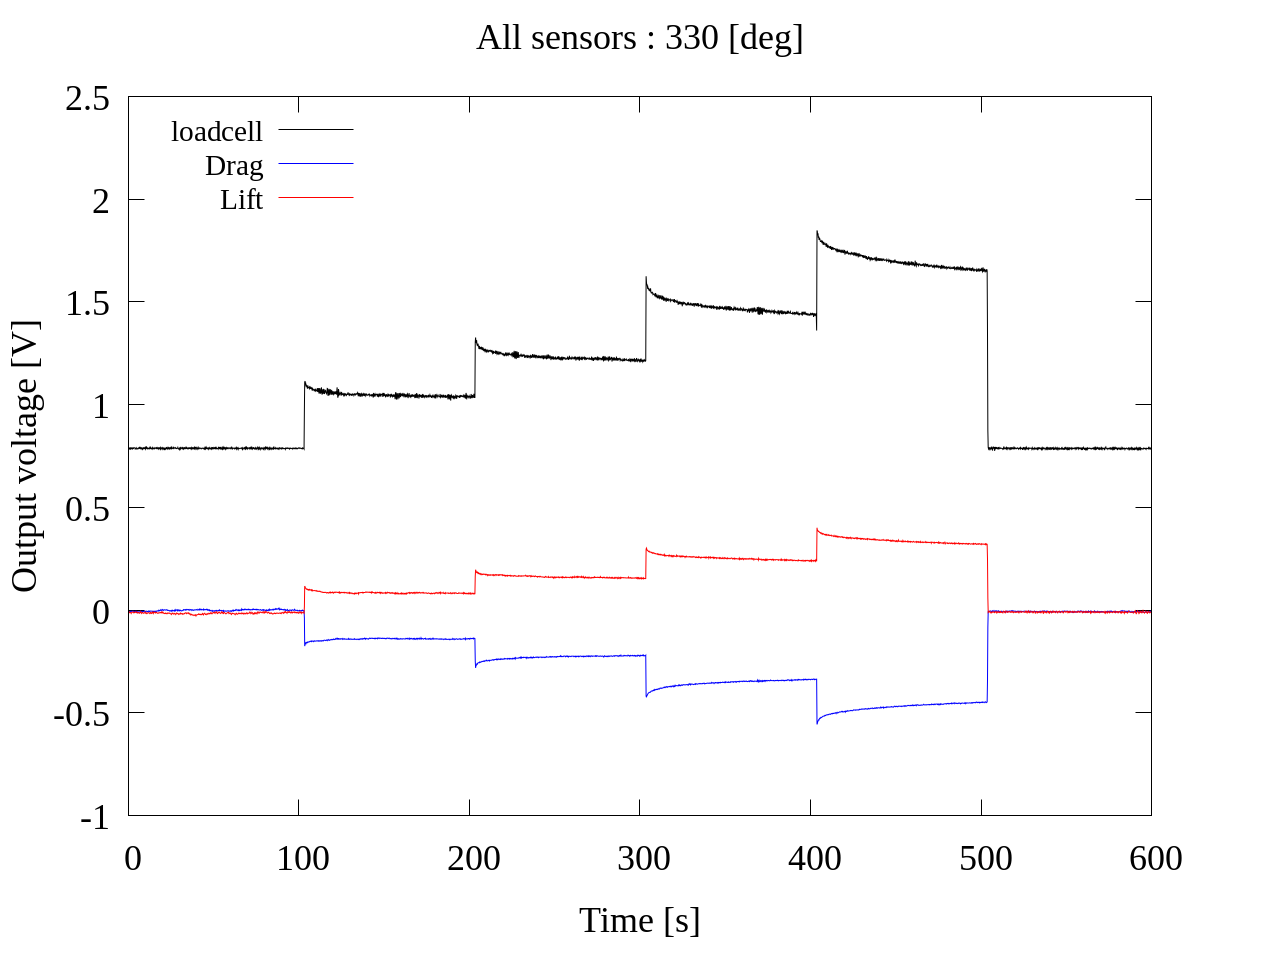
\includegraphics[width=78mm]{../images/330.png}
        \caption{Acting force from 330 degree direction}
    \end{center}
\end{figure}

\newpage
\;
\newpage
\;
\newpage

\subsection{作用力の角度と出力電圧の傾きの関係}

Fig.23~34について,抗力・揚力のそれぞれの近似直線の傾きと
作用力方向の関係について以下のTable.1,Fig.35に示す.\\
また,作用力方向の違いによって出力電圧にどのような影響があるかを調べるため,
以下のように抗力と揚力の勾配比を算出した.\\

\begin{itembox}[l]{抗力・揚力の勾配比}
    \begin{center}
        $\displaystyle \left(L/D:勾配比\right) = $
        \vskip\baselineskip
        $\displaystyle \left|\frac{\left(L:揚力側出力電圧の近似直線の傾き\right)}{\left(D:抗力側出力電圧の近似直線の傾き\right)}\right|$
    \end{center}
\end{itembox}

\begin{figure}[htbp]
    \footnotesize
    \begin{center}
        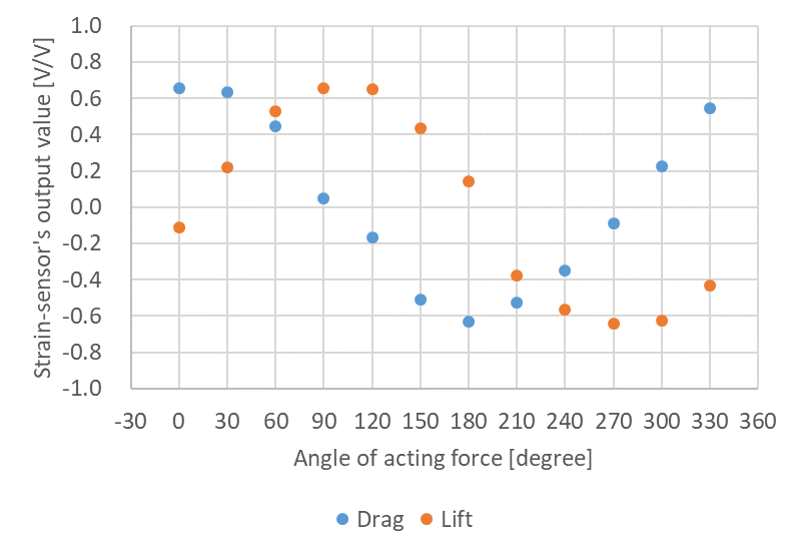
\includegraphics[width=85mm]{../images/experiment_results.png}
        \caption{Experiment results}
    \end{center}
\end{figure}

\begin{table}[htbp]
    \caption{Experiment results of gradient ratio}
    \begin{center}
        \begin{tabular}{|p{20mm}|p{20mm}|p{20mm}|p{20mm}|}
            \hline
            \multicolumn{1}{|c|}{\textgt{Angle [deg]}} & \multicolumn{1}{|c|}{\textgt{D [V/V]}} & \multicolumn{1}{|c|}{\textgt{L [V/V]}} & \multicolumn{1}{|c|}{\textgt{L/D [-]}} \\ \hline
            \multicolumn{1}{|c|}{0}                    & \multicolumn{1}{|c|}{0.656}            & \multicolumn{1}{|c|}{-0.110}           & \multicolumn{1}{|c|}{0.168}            \\ \hline
            \multicolumn{1}{|c|}{30}                   & \multicolumn{1}{|c|}{0.632}            & \multicolumn{1}{|c|}{0.221}            & \multicolumn{1}{|c|}{0.349}            \\ \hline
            \multicolumn{1}{|c|}{60}                   & \multicolumn{1}{|c|}{0.448}            & \multicolumn{1}{|c|}{0.530}            & \multicolumn{1}{|c|}{1.182}            \\ \hline
            \multicolumn{1}{|c|}{90}                   & \multicolumn{1}{|c|}{0.048}            & \multicolumn{1}{|c|}{0.657}            & \multicolumn{1}{|c|}{13.688}           \\ \hline
            \multicolumn{1}{|c|}{120}                  & \multicolumn{1}{|c|}{-0.169}           & \multicolumn{1}{|c|}{0.653}            & \multicolumn{1}{|c|}{3.861}            \\ \hline
            \multicolumn{1}{|c|}{150}                  & \multicolumn{1}{|c|}{-0.510}           & \multicolumn{1}{|c|}{0.437}            & \multicolumn{1}{|c|}{0.856}            \\ \hline
            \multicolumn{1}{|c|}{180}                  & \multicolumn{1}{|c|}{-0.632}           & \multicolumn{1}{|c|}{0.142}            & \multicolumn{1}{|c|}{0.224}            \\ \hline
            \multicolumn{1}{|c|}{210}                  & \multicolumn{1}{|c|}{-0.527}           & \multicolumn{1}{|c|}{-0.380}           & \multicolumn{1}{|c|}{0.720}            \\ \hline
            \multicolumn{1}{|c|}{240}                  & \multicolumn{1}{|c|}{-0.350}           & \multicolumn{1}{|c|}{-0.564}           & \multicolumn{1}{|c|}{1.611}            \\ \hline
            \multicolumn{1}{|c|}{270}                  & \multicolumn{1}{|c|}{-0.088}           & \multicolumn{1}{|c|}{-0.642}           & \multicolumn{1}{|c|}{7.282}            \\ \hline
            \multicolumn{1}{|c|}{300}                  & \multicolumn{1}{|c|}{0.226}            & \multicolumn{1}{|c|}{-0.625}           & \multicolumn{1}{|c|}{2.771}            \\ \hline
            \multicolumn{1}{|c|}{330}                  & \multicolumn{1}{|c|}{0.546}            & \multicolumn{1}{|c|}{-0.431}           & \multicolumn{1}{|c|}{0.789}            \\ \hline
        \end{tabular}
    \end{center}
\end{table}

\newpage

\subsection{理論値との比較}

理論上の勾配比についても以下のように算出した.
作用力ベクトルの大きさを1として,それぞれの角度(30度ごと)に供試体に作用したときに加わる作用力ベクトルの長さを
抗力・揚力方向について算出し,その比をとることで理想的な作用力の比,すなわち勾配比を算出することができる.
以下のTable.2にその算出結果を示す。\par

\begin{table}[htbp]
    \caption{Calucuration of gradient ratio}
    \begin{center}
        \begin{tabular}{|p{20mm}|p{20mm}|p{20mm}|p{20mm}|}
            \hline
            \multicolumn{1}{|c|}{\textgt{Angle [deg]}} & \multicolumn{1}{|c|}{\textgt{  Drag [-]  }} & \multicolumn{1}{|c|}{\textgt{  Lift [-]  }} & \multicolumn{1}{|c|}{\textgt{  L/D [-]  }} \\ \hline
            \multicolumn{1}{|c|}{0}                    & \multicolumn{1}{|c|}{1.000}                 & \multicolumn{1}{|c|}{0.000}                 & \multicolumn{1}{|c|}{0.000}                \\ \hline
            \multicolumn{1}{|c|}{30}                   & \multicolumn{1}{|c|}{0.870}                 & \multicolumn{1}{|c|}{0.500}                 & \multicolumn{1}{|c|}{0.580}                \\ \hline
            \multicolumn{1}{|c|}{60}                   & \multicolumn{1}{|c|}{0.500}                 & \multicolumn{1}{|c|}{0.870}                 & \multicolumn{1}{|c|}{1.730}                \\ \hline
            \multicolumn{1}{|c|}{90}                   & \multicolumn{1}{|c|}{0.000}                 & \multicolumn{1}{|c|}{1.000}                 & \multicolumn{1}{|c|}{$\infty$}             \\ \hline
            \multicolumn{1}{|c|}{120}                  & \multicolumn{1}{|c|}{-0.500}                & \multicolumn{1}{|c|}{0.870}                 & \multicolumn{1}{|c|}{1.730}                \\ \hline
            \multicolumn{1}{|c|}{150}                  & \multicolumn{1}{|c|}{-0.870}                & \multicolumn{1}{|c|}{0.500}                 & \multicolumn{1}{|c|}{0.580}                \\ \hline
            \multicolumn{1}{|c|}{180}                  & \multicolumn{1}{|c|}{-1.000}                & \multicolumn{1}{|c|}{0.000}                 & \multicolumn{1}{|c|}{0.000}                \\ \hline
            \multicolumn{1}{|c|}{210}                  & \multicolumn{1}{|c|}{-0.870}                & \multicolumn{1}{|c|}{-0.500}                & \multicolumn{1}{|c|}{0.580}                \\ \hline
            \multicolumn{1}{|c|}{240}                  & \multicolumn{1}{|c|}{-0.500}                & \multicolumn{1}{|c|}{-0.870}                & \multicolumn{1}{|c|}{1.730}                \\ \hline
            \multicolumn{1}{|c|}{270}                  & \multicolumn{1}{|c|}{0.000}                 & \multicolumn{1}{|c|}{-1.000}                & \multicolumn{1}{|c|}{$\infty$}             \\ \hline
            \multicolumn{1}{|c|}{300}                  & \multicolumn{1}{|c|}{0.500}                 & \multicolumn{1}{|c|}{-0.870}                & \multicolumn{1}{|c|}{1.730}                \\ \hline
            \multicolumn{1}{|c|}{330}                  & \multicolumn{1}{|c|}{0.870}                 & \multicolumn{1}{|c|}{-0.500}                & \multicolumn{1}{|c|}{0.580}                \\ \hline
        \end{tabular}
        \vskip\baselineskip
        \small{※ Drag 及び Lift は,作用力ベクトルの大きさ[-]を表す}
    \end{center}
\end{table}

Table.1及びTable.2の$L/D$算出結果の関係を以下のFig.36に示す.

\begin{figure}[htbp]
    \footnotesize
    \begin{center}
        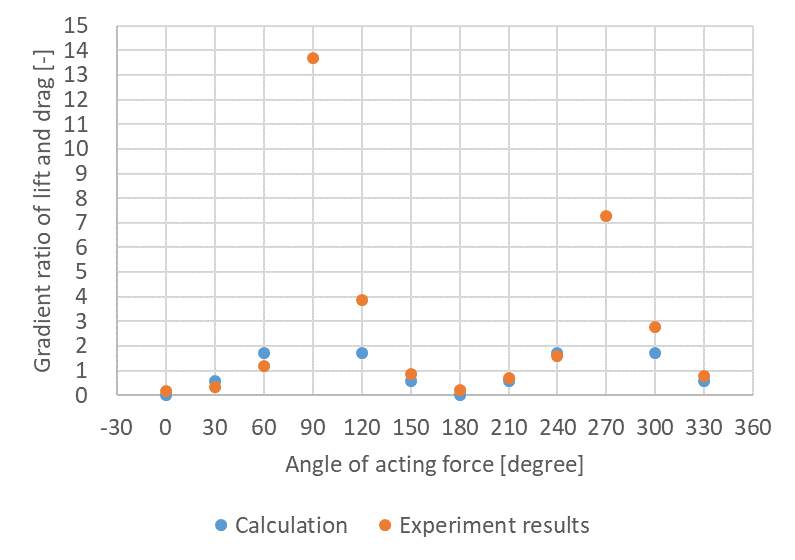
\includegraphics[width=85mm]{../images/gradient_ratio_2.png}
        \caption{Gradient ratio of lift and drag}
    \end{center}
\end{figure}

\section{実験装置のたわみ量とひずみの算出}
    試験用のひずみセンサを選定するにあたり,
    ひずみセンサの取付部の作用力によるひずみ量を調べる必要がある.
    ここで,簡単のため可能な限り切りのいい数字を使っておおよその変位量を算出した.\\

\subsection{算出結果}
\begin{screen}
    \begin{itemize}
        \item 先端のたわみ量  :$0.151 \;\left[\mathrm{mm}\right]$
        \item 取付軸表面の伸縮量:$1.029 × 10^{-3} \;\left[\mathrm{mm}\right]$
        \item 取付軸表面のひずみ:$5.717 × 10^{-6} \left[\mathrm{-}\right]$
    \end{itemize}
\end{screen}

\subsection{算出条件}
\begin{screen}
    \begin{itemize}
        \item [$\bullet$] アルミニウムの弾性係数  :$E = 70 \left[\mathrm{GPa}\right]$
        \item [$\bullet$] ひずみセンサと作用点の距離:$l_1 = 725 \left[\mathrm{mm}\right]$
        \item [$\bullet$] 取付部材料の長さ     :$l_2 = 180 \left[\mathrm{mm}\right]$
        \item [$\bullet$] 作用力          :$F = 0.15 \left[\mathrm{N}\right]$
        \item [$\bullet$] 断面二次モーメント    :$I = 2701 \left[\mathrm{mm^4}\right]$
        \item [$\bullet$] 取付部に加わるモーメント :$M$
        \item [$\bullet$] 取付部のたわみの曲率半径 :$R$
        \item [$\bullet$] 取付部のたわみ角     :$\theta$
        \item [$\bullet$] 取付部のたわみ      :$w$
        \item [$\bullet$] 取付部表面の伸び     :$\lambda$
        \item [$\bullet$] 取付部表面のひずみ    :$\varepsilon$
        \item [$\bullet$] 取付部表面と中立軸の距離 :$\delta r$
    \end{itemize}
\end{screen}

\begin{figure}[htbp]
    \footnotesize
    \begin{center}
        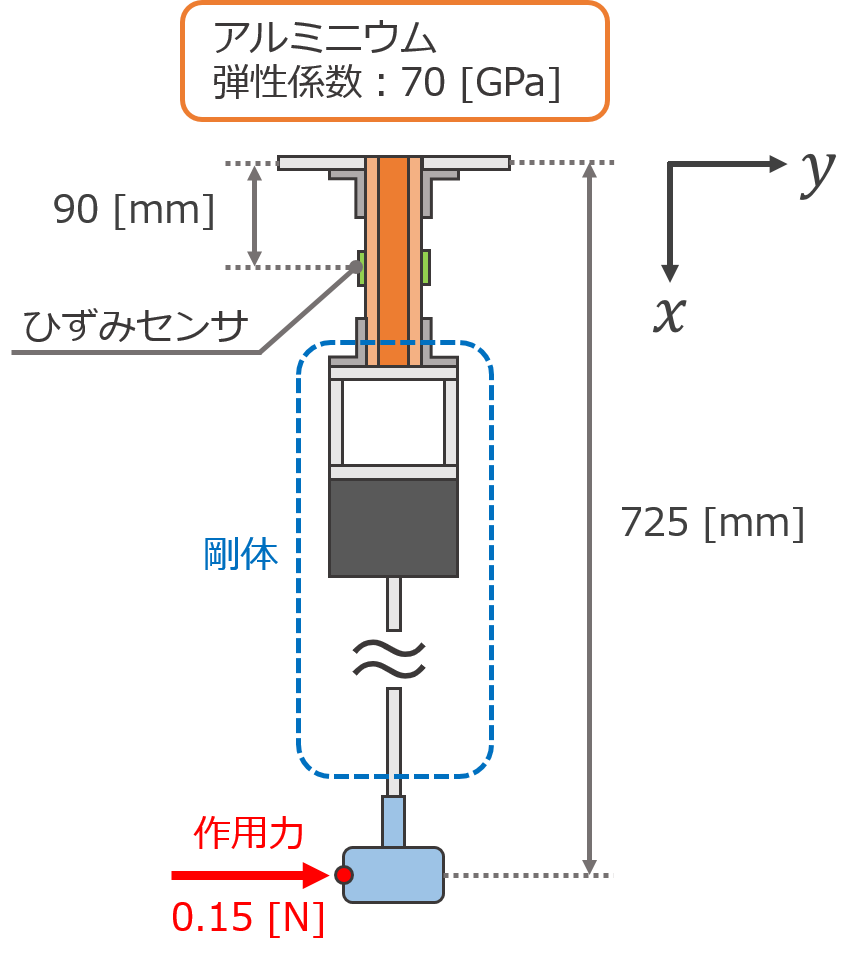
\includegraphics[width=70mm]{../images/moment.png}
        \caption{Cross-sectional shape of experimental device}
    \end{center}
\end{figure}

\subsubsection{算出過程}
\begin{itemize}
    \item [$\blacksquare$] 実験装置に加わるモーメントの算出
    \begin{eqnarray*}
        M &=& F × \frac{l_1}{1000}\\
        &=& 0.15 × 0.725\\
        &=& 0.10875 \;\left[\mathrm{N \cdot m}\right]
    \end{eqnarray*}
    \item [$\blacksquare$] たわみの曲率半径の算出
    \begin{itembox}[l]{たわみの曲率半径}
        \begin{center}
            $\displaystyle \frac{1}{R} = \frac{M}{EI}$
        \end{center}
    \end{itembox}
    \begin{eqnarray*}
        R &=& \frac{EI}{M}\\
        &=& 70 × 2701 × \frac{100000}{10875}\\
        &\approx& 1738577.713 \left[\mathrm{mm}\right]
    \end{eqnarray*}
    \item [$\blacksquare$] 位置$x$[mm] におけるたわみ角とたわみの算出
    \begin{itembox}[l]{たわみの微分方程式}
            \begin{center}
                $\displaystyle \frac{d^2w}{dx^2}=-\frac{M}{EI}$\\
                \vskip\baselineskip
                ※ 今回のひずみは正の値となる
            \end{center}
    \end{itembox}
    \begin{itembox}[l]{初期条件}
    \begin{itemize}
        \item [$\bullet$] $x=0$ のとき $w=0$,$\theta =0$
    \end{itemize}
    \end{itembox}
    \begin{eqnarray*}
        \frac{d^2w}{dx^2}&=&\frac{M}{EI}\\
        &=&\frac{0.10875}{70 × 2701}\\
        &=&5.7518 \cdots × 10^{-7}\\
        &\approx& 5.752 × 10^{-7} \;\left[\mathrm{1/mm}\right]\\ \\
        \frac{dw}{dx} &=& \theta = \frac{M}{EI} x + C_1\\ \\
        w &=& \frac{1}{2} \frac{M}{EI} x^2 + C_1x + C_2
    \end{eqnarray*}
    初期条件より
    \begin{eqnarray*}
        C_1 = C_2 = 0
    \end{eqnarray*}
    したがって,
    \begin{eqnarray*}
        \theta &=& \frac{M}{EI}x\\ \\
        w &=& \frac{1}{2}\frac{M}{EI}x^2\\
    \end{eqnarray*}
        \item [$\blacksquare$] ひずみセンサ取付部($x=90$)の伸びの算出\\
    $x = 90$のとき,たわみ角は,
    \begin{eqnarray*}
        \theta &=& \frac{M}{EI} × 90\\
        &=& 5.7152 × 10^{-7} × 90\\
        &=& 5.1437 × 10^{-5}\\
        &\approx& 5.144 × 10^{-5} \;\left[\mathrm{rad}\right]
    \end{eqnarray*}
    したがって,取付軸の伸び$\lambda$は,
    \begin{eqnarray*}
        \lambda &=& \left(R+\delta r\right)\theta - R\theta\\
        &=& \delta r \theta\\
        &=& 10 × \;\theta\\
        &=& 10 × 5.1437 × 10^{-5}\\
        &=& 5.1437 × 10^{-4}\\
        &\approx& 5.144 × 10^{-4} \;\left[\mathrm{mm}\right]\\
    \end{eqnarray*}
    \item [$\blacksquare$] ひずみセンサ取付部($x=90$)のひずみの算出
        \begin{eqnarray*}
            \varepsilon &=& \frac{\lambda}{l_2}\\
            &=& \frac{5.144 × 10^{-4}}{180}\\
            &=& 2.8577 × 10^{-6}\cdots\\
            &\approx& 2.858 × 10^{-6} \left[\mathrm{-}\right]
        \end{eqnarray*}
    \item [$\blacksquare$] 先端($x=725$)のたわみ量 $w$ の算出
    \begin{eqnarray*}
        w &=& \frac{1}{2} × \frac{M}{EI} × l^2\\
        &=& \frac{1}{2} × 5.752 × 10^{-7} × 725^2\\
        &=& 0.1511 \cdots\\
        &\approx& 0.151 \;\left[\mathrm{mm}\right]
    \end{eqnarray*}
\end{itemize}

\subsection{ひずみ量の算出式の作成}

\subsubsection{算出過程}
\begin{eqnarray*}
    \varepsilon &=& \frac{\lambda}{l_2}\\
    &=& \frac{\theta}{l_2} × \delta r\\
    &=& \frac{M × 90}{l_2 × EI} × \delta r\\
    &=& \frac{l_1 × 90}{1000 × l_2 × EI} × F × \delta r\\
    &=& \frac{725 × 90}{1000 × 180 × 70 × 2701} × F × \delta r\\
    &=& 1.9172 \cdots × 10^{-6} × F × \delta r\\
    &\approx& 1.917 × 10^{-6} × F × \delta r\\
\end{eqnarray*}

\begin{itembox}[l]{ひずみ量の算出式}
    \begin{center}
        $\displaystyle \varepsilon = 1.197 × 10^{-6} × F × \delta r$
    \end{center}
\end{itembox}

また,取付部表面と中立軸の距離:$\delta r$について
比較形状ごとの値を以下に示す.

% \begin{itembox}[l]{比較形状の寸法}
%     \begin{enumerate}[(i)]
%         \item 円筒 : $D_1=\;$20.0 [mm],$D_2=\;$18.0 [mm]
%         \item 円柱 : $D=\;$15.3 [mm]
%         \item 角柱 : $L=\;$13.4 [mm]
%     \end{enumerate}
% \end{itembox}

\begin{itembox}[l]{取付部表面と中立軸の距離}
    \begin{enumerate}[(i)]
        \item 円筒 : $\delta r_1 = 10.0$ [mm]
        \item 円柱 : $\delta r_2 = 7.65$ [mm]
        \item 角柱 : $\delta r_3 = 6.70$ [mm]
    \end{enumerate}
\end{itembox}

したがって,実験装置に加えられる作用力を 1 [N] と仮定し,
それぞれの比較形状についてひずみを算出すると,以下のようになる.

\begin{itembox}[l]{各試験片のひずみ量}
    \begin{enumerate}[(i)]
        \item 円筒 : $\varepsilon_1 \approx 1.197 × 10^{-5}$ [-]
        \item 円柱 : $\varepsilon_2 \approx 1.467 × 10^{-5}$ [-]
        \item 角柱 : $\varepsilon_3 \approx 1.284 × 10^{-5}$ [-]
    \end{enumerate}
\end{itembox}

\newpage

\section{ひずみゲージの選定}

\subsection{現在使用しているロードセルについて}
現在使用しているロードセルについての情報を以下に示す.

\begin{screen}
    \begin{itemize}
        \item [$\bullet$]   名称  : 微小荷重圧縮引張型 UTA
        \item [$\bullet$]   型番  : UTA-100GR
        \item [$\bullet$]  定格容量 : $0.9807 ~ 19.61 \left[\mathrm{N}\right]$
        \item [$\bullet$] 推奨印可電圧: 3V 以下
    \end{itemize}
\end{screen}

\end{document}